\subsection{2D Convection-Diffusion - Smith-Hutton Case}~\label{secConvection2D}
The Smith-Hutton problem~\cite{SmithHutton1982} is a widely used benchmark for convection-diffusion schemes. It consists of a rectangular domain $[-1, 1] \times [0, 1]$ subject to a prescribed, analytically divergence-free velocity field:

\begin{equation}~\label{eqSHVelocity}
    u = 2y(1 - x^2), \qquad v = -2x(1 - y^2)
\end{equation}

This velocity field generates a circular flow that enters along the bottom from the left, sweeps across the domain, curves upward near the east boundary, and returns from right to left along the top. Because $\nabla \cdot \mathbf{v} = 0$ is satisfied analytically, the discrete continuity correction term in Eq.~\eqref{eqConv_ap} vanishes exactly, making this a clean test of the convective discretisation alone. A schematic of the problem is shown in Fig.~\ref{figSHDomain}.

\begin{figure}[ht]
    \centering
    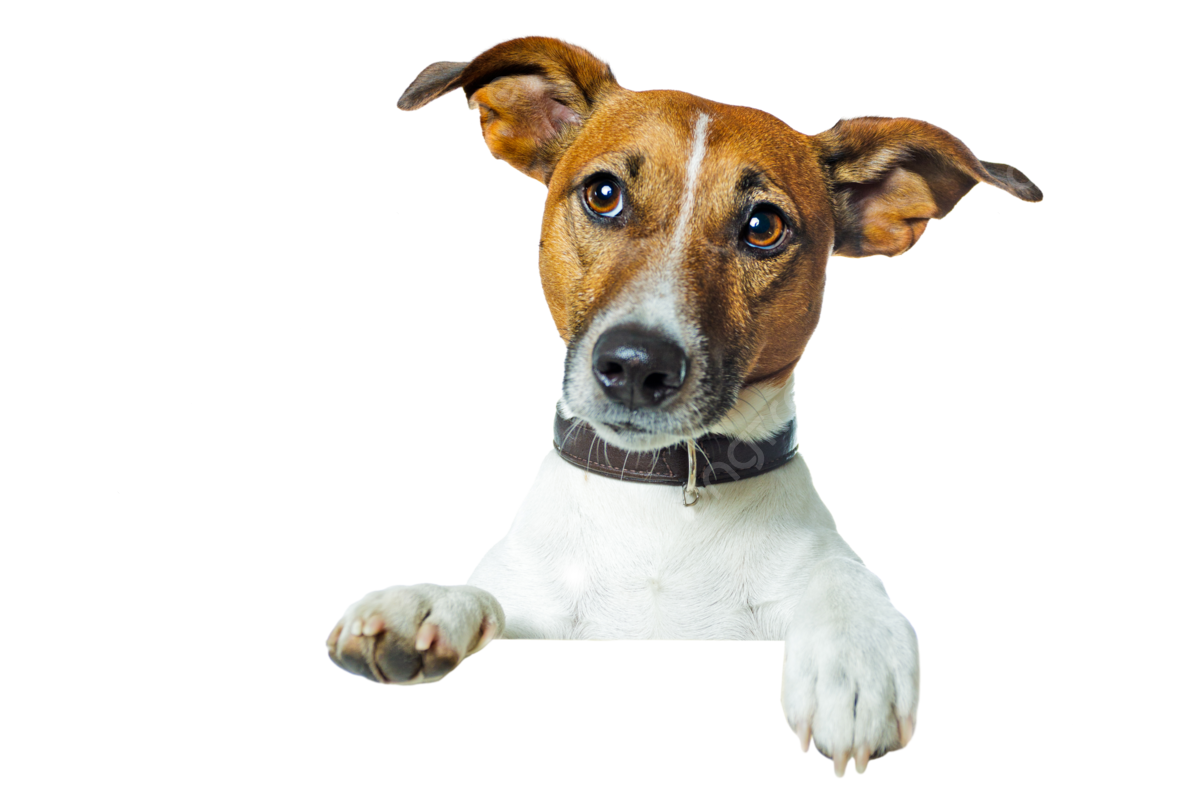
\includegraphics[width=0.45\linewidth]{Chapter2/Media/PLACEHOLDER.png}
    \caption{Smith-Hutton problem domain and velocity streamlines~\cite{SmithHutton1982}.}
    \label{figSHDomain}
\end{figure}

The transport variable $\phi$ represents a passive scalar carried by the flow. Boundary conditions are:

\begin{itemize}
    \item \textbf{South inlet} ($y = 0,\ -1 \leq x \leq 0$): Dirichlet profile $\phi = 1 + \tanh\!\bigl(10(2x + 1)\bigr)$, which ramps from $0$ at $x = -1$ through $1$ at $x = -0.5$ to $2$ at $x = 0$.
    \item \textbf{South outlet} ($y = 0,\ 0 \leq x \leq 1$): Neumann zero-gradient $\partial \phi / \partial n = 0$.
    \item \textbf{All remaining walls}: Dirichlet $\phi = 0$.
\end{itemize}

The steep inlet profile makes this a demanding benchmark: a high-order scheme must resolve the sharp gradient without introducing oscillations, while an upwind scheme will smear it due to numerical diffusion. The problem is parameterised by the ratio $\rho/\Gamma$, which controls the global Peclet number. Three cases are tested: $\rho/\Gamma = 10^1$, $10^3$, and $10^6$, with $\Gamma = 1$ held fixed throughout. Validation is performed by comparing the computed exit profile $\phi(x,\, y=0)$ for $0 \leq x \leq 1$ against the reference values provided by Smith and Hutton~\cite{SmithHutton1982}.


\subsubsection{Model Implementation}
The convection-diffusion solver is built on the same modular architecture as Chapter~\ref{chapDiffusion}, extending it with three key additions. First, the velocity field is no longer a fixed parameter but a prescribed analytical input: the two components $u$ and $v$ are specified as mathematical expressions in the configuration file, which are parsed and evaluated at each cell face during the assembly of the convective fluxes $F_k$. This approach keeps the model general, allowing any analytically defined, divergence-free velocity field to be tested without modifying the source code. Second, ghost nodes are used at all domain boundaries (see Section~\ref{chapConvection}) instead of the half-cell wall treatment of Chapter~\ref{chapDiffusion}, enabling a consistent treatment of both the diffusive and convective face fluxes. Third, a new Boundary probe type was added to the Probe class, which records $\phi$ along a specified boundary face at each saved time-step; this is required for the Smith-Hutton validation, which compares the exit profile at the south outlet.

A summary of all configuration parameters for this model is shown in Table~\ref{tabConfigConv}. Compared to the previous chapter, the main additions are the \textbf{spatScheme} parameter for the convective scheme, the \textbf{velocityField} entry for the analytical velocity expressions, and the \textbf{medicOn} flag that activates the diagnostic tool.

\begin{table}[ht]
	\centering
	\begin{tabular}{|l|c|p{0.5\linewidth}|}
		\hline
		Group & Parameter & Description \\
		\hline
		\multirow{8}{*}{Numerical Data} & tempScheme & Temporal scheme selection for simulation. \\
            & spatScheme & Convective scheme selection for simulation. \\
            & solver & Solver algorithm for simulation. \\
			& tolNumeric & Tolerance for the numerical solver. \\
			& tolTemporal & Tolerance for the steady-state convergence. \\
			& maxIterations & Limit of iterations per time-step. \\
			& endTime & Last instant of the simulation. \\
			& timeStep & Time increment after each instant. \\
		\hline
		\multirow{4}{*}{Physical Data} & T0 & Initial value for $\phi$ over the domain. \\
					       & \multirow{2}{*}{materials} & List of vectors with thermophysical properties corresponding to each material. \\
                           & velocityField & Mathematical expressions for each velocity component. \\
		\hline
		\multirow{5}{*}{Geometrical Data} & width & Dimension of the domain in the secondary axis. \\
						  & \multirow{4}{*}{sections} & List of vectors indicating the material distribution. Also includes node count and internal source. \\
		\hline
		\multirow{9}{*}{Mesh Data} & strength & Cubic algebraic mesh parameter. \\
					   & centering & Cubic algebraic mesh parameter. \\
					   & kappa & Power law mesh parameter. \\
					   & delta & Hyperbolic tangent mesh parameter. \\
					   & meshAlgorithm & Algorithm for mesh generation. \\
					   & \multirow{2}{*}{N} & List specifying total number of nodes for each axis. \\
					   & \multirow{2}{*}{refinement} & List of vectors specifying refinement configuration for each axis. \\
		\hline
		\multirow{2}{*}{Boundary Data} & \multirow{2}{*}{boundaries} & List of vectors specifying the boundary conditions on each side. \\
		\hline
		\multirow{2}{*}{Probe Data} & \multirow{2}{*}{probes} & List of vectors specifying the probes configured for the simulation. \\
		\hline
        Medic Data & medicOn & Control argument for the diagnostic tool. \\
        \hline
	\end{tabular}
	\caption{Configuration file structure for the convection-diffusion model, highlighting the new parameters introduced in this chapter.}
	\label{tabConfigConv}
\end{table}


\subsubsection{BiCGSTAB Solver}
The introduction of the convective term breaks the symmetry of the coefficient matrix $A$: the upwind contribution to $a_W$ is not equal to the corresponding entry in $a_E$, so $A \neq A^T$ in general. The Conjugate Gradient method requires a symmetric positive-definite system and therefore is no longer applicable once the convective term is present. The BiConjugate Gradient Stabilized (BiCGSTAB) method~\cite{vanderVorst1992} extends the Krylov subspace approach to general non-symmetric systems by maintaining two coupled residual sequences. The method introduces a shadow residual $\hat{\mathbf{r}}$, fixed at the initial residual $\mathbf{r}^0$ and never updated, which provides a stable projection direction throughout the iteration. Each step of the algorithm contains two substeps: a standard BiCG step that computes a step length $\alpha_k$, and a local minimisation step controlled by $\omega_k$ that minimises the residual along the direction $A\mathbf{s}^k$. This suppresses the irregular convergence oscillations that characterise standard BiCG and gives the method its stabilised name. Algorithm~\ref{algBiCGSTAB} summarises the procedure.

\begin{algorithm}[ht]
\caption{BiConjugate Gradient Stabilized (BiCGSTAB) solver}
\label{algBiCGSTAB}
\begin{algorithmic}[1]
    \Require Non-singular matrix $A$, RHS vector $\mathbf{b}$, initial guess $\boldsymbol{\phi}^0$, tolerance $\varepsilon$, maximum iterations $k_{\max}$
    \Ensure Solution vector $\boldsymbol{\phi}$
    \State $\mathbf{r}^0 \gets \mathbf{b} - A\boldsymbol{\phi}^0$;\quad $\hat{\mathbf{r}} \gets \mathbf{r}^0$;\quad $\mathbf{p}^0 \gets \mathbf{r}^0$;\quad $\boldsymbol{\phi} \gets \boldsymbol{\phi}^0$
    \For{$k = 0, 1, 2, \ldots, k_{\max}$}
        \State $\alpha_k \gets \dfrac{\hat{\mathbf{r}} \cdot \mathbf{r}^k}{\hat{\mathbf{r}} \cdot A\mathbf{p}^k}$
        \State $\mathbf{s}^k \gets \mathbf{r}^k - \alpha_k A\mathbf{p}^k$
        \If{$\|\mathbf{s}^k\| < \varepsilon$}
            \State $\boldsymbol{\phi} \gets \boldsymbol{\phi}^k + \alpha_k\mathbf{p}^k$;\quad \textbf{break}
        \EndIf
        \State $\omega_k \gets \dfrac{(A\mathbf{s}^k) \cdot \mathbf{s}^k}{\|A\mathbf{s}^k\|^2}$
        \State $\boldsymbol{\phi}^{k+1} \gets \boldsymbol{\phi}^k + \alpha_k\mathbf{p}^k + \omega_k\mathbf{s}^k$
        \State $\mathbf{r}^{k+1} \gets \mathbf{s}^k - \omega_k A\mathbf{s}^k$
        \If{$\|\mathbf{r}^{k+1}\| < \varepsilon$}
            \State \textbf{break}
        \EndIf
        \State $\beta_k \gets \dfrac{\hat{\mathbf{r}} \cdot \mathbf{r}^{k+1}}{\hat{\mathbf{r}} \cdot \mathbf{r}^k} \cdot \dfrac{\alpha_k}{\omega_k}$
        \State $\mathbf{p}^{k+1} \gets \mathbf{r}^{k+1} + \beta_k(\mathbf{p}^k - \omega_k A\mathbf{p}^k)$
    \EndFor
    \Return $\boldsymbol{\phi}$
\end{algorithmic}
\end{algorithm}

Like CG, BiCGSTAB is a Krylov method and converges in at most $N$ iterations for an $N \times N$ system, though in practice convergence is reached much earlier. The cost per iteration is higher than CG — two matrix-vector products per step instead of one — but this is outweighed by the ability to handle the asymmetric systems that arise whenever convection is present. As explained in Chapter~\ref{chapNavierStokes}, the same solver is carried forward to the Navier-Stokes model.


\subsubsection{Numerical Parameter Study}
Before the full scheme comparison can be run under controlled conditions, a working mesh resolution must be established. The mesh refinement study described below uses the Smith-Hutton problem with the UDS scheme and $\rho/\Gamma = 10^3$ as the base case, sweeping the number of nodes $N$ across four levels. The chosen resolution is then used for all subsequent validation runs. A summary of the tested values is shown in Table~\ref{tabConvNumerical}.

\begin{table}[ht]
    \centering
    \begin{tabular}{|c|c|}
        \hline
        Parameter & Values \\
        \hline
        $N$ & 16,\ 32,\ \textbf{64},\ 128 \\
        \hline
    \end{tabular}
    \caption{Mesh sizes tested in the spatial refinement study. The bold value indicates the resolution selected for validation.}
    \label{tabConvNumerical}
\end{table}

\paragraph{Mesh Refinement}
The Smith-Hutton problem is solved at four progressively finer uniform meshes using the Hybrid scheme and $\rho/\Gamma = 10^3$. Since no closed-form analytical solution exists, the $L_2$ error of the exit profile $\phi(x,\, y=0)$ for $0 \leq x \leq 1$ is computed against the reference values of Smith and Hutton~\cite{SmithHutton1982}:

\begin{equation}~\label{eqSHL2}
    e_N = \left\| \phi_{\mathrm{num}} - \phi_{\mathrm{ref}} \right\|_2 = \sqrt{\frac{1}{N_{\mathrm{out}}} \sum_{i} (\phi_i - \phi_{\mathrm{ref},i})^2}
\end{equation}

where $N_{\mathrm{out}}$ is the number of outlet nodes used in the comparison. The left panel of Fig.~\ref{figConvRefinement} shows the evolution of the exit profile as $N$ increases; the right panel is a log-log plot of $e_N$ against the mesh spacing $h = 2/N_x$, from which the spatial order of convergence can be read off by comparing against the reference slope lines.

\begin{figure}[ht]
    \centering
    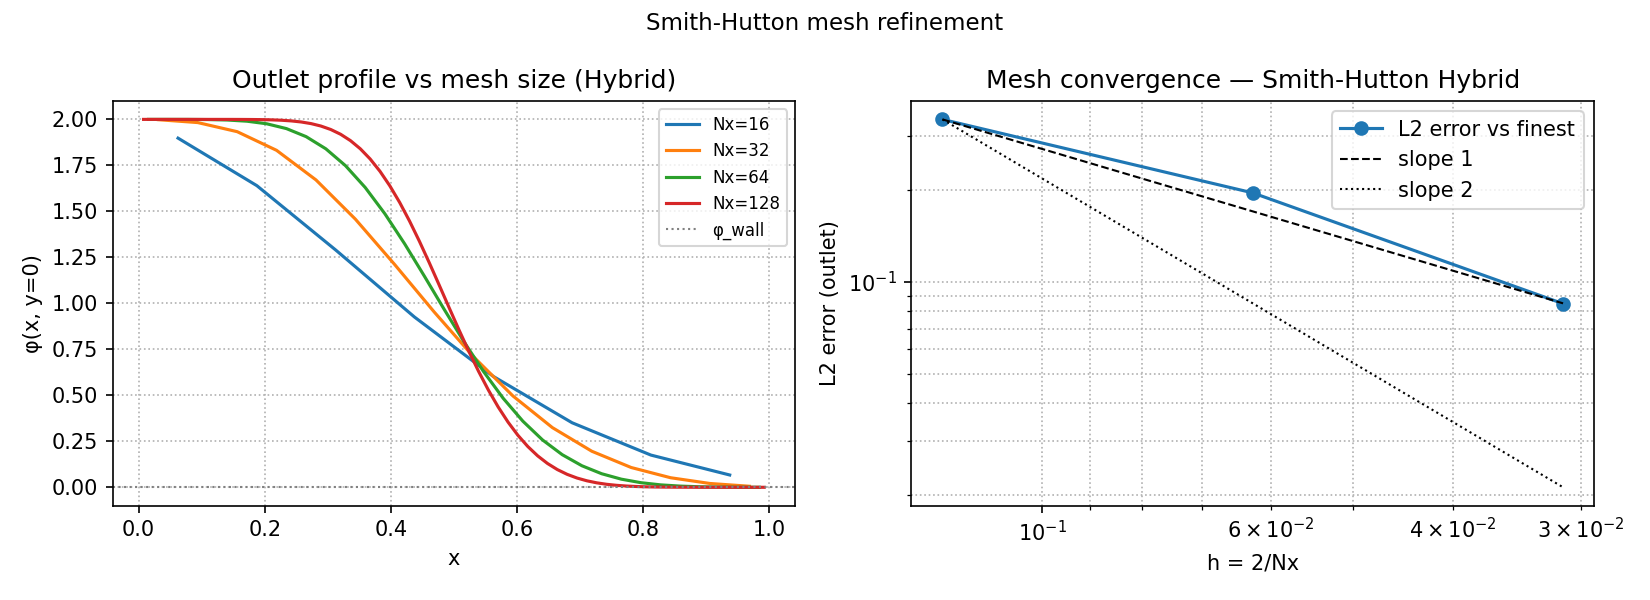
\includegraphics[width=\linewidth]{Chapter2/Media/SHRefine.png}
    \caption{Mesh refinement study for the Smith-Hutton case ($\rho/\Gamma = 10^3$, Hybrid). Left: exit profile $\phi(x, 0)$ for each mesh level. Right: $L_2$ error against mesh spacing $h = 2/N_x$; reference slope lines indicate first- and second-order convergence rates.}
    \label{figConvRefinement}
\end{figure}


\subsubsection{Model Validation}
The model is validated by running the Smith-Hutton problem for three convective schemes — CDS, UDS, and Hybrid — across all three values of $\rho/\Gamma$, using the mesh resolution established by the refinement study. The three schemes represent different points in the accuracy-stability trade-off described in Table~\ref{tabConvSchemes}: CDS is second-order accurate but loses diagonal dominance for $|Pe_k| > 2$, which causes oscillations; UDS maintains diagonal dominance at all Peclet numbers but is only first-order accurate; and the Hybrid scheme applies CDS where $|Pe_k| \leq 2$ and switches to UDS above that threshold. This range of behaviours is expected to produce clearly different exit profiles as $\rho/\Gamma$ increases and convection becomes dominant.

For each $\rho/\Gamma$ case, two quantities are reported: the number of inner solver iterations and the final residual, which assess convergence and stability; and the exit profile $\phi(x,\, y=0)$, which is compared directly against the reference values~\cite{SmithHutton1982}. The steady-state $\phi$ colormaps for all three schemes are also provided to give a visual assessment of the transport behaviour and to expose the CDS divergence at high Peclet numbers. The results are presented in Figs.~\ref{figConvNumerical},~\ref{figConvSH}, and~\ref{figConvUDS}.

\begin{figure}[ht]
    \centering
    \begin{tabular}{cc}
        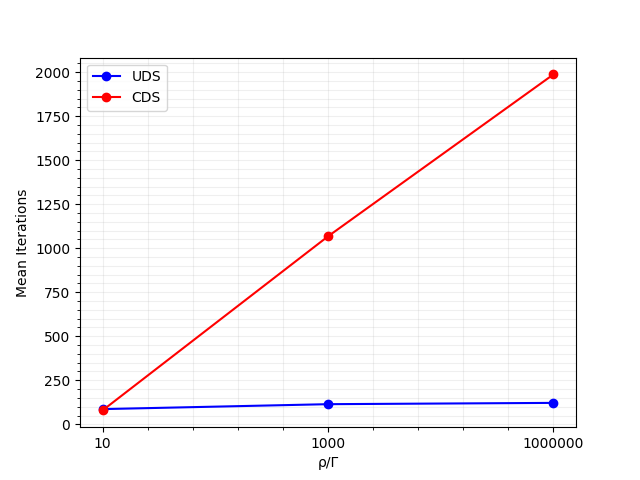
\includegraphics[width=0.45\linewidth]{Chapter2/Media/IterConv.png} & 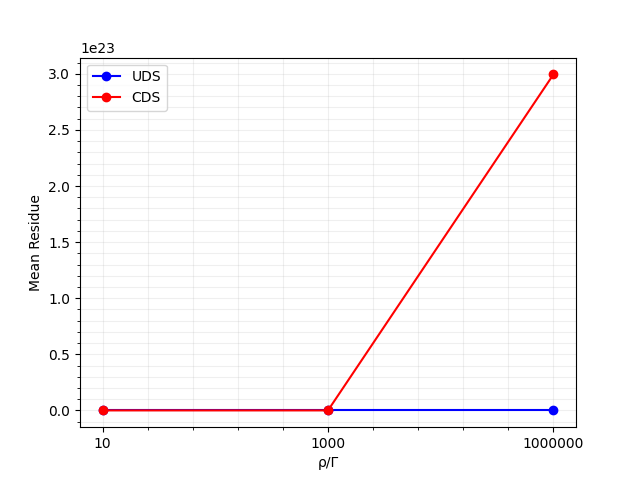
\includegraphics[width=0.45\linewidth]{Chapter2/Media/ResidueConv.png} \\
    \end{tabular}
    \caption{Number of iterations (left) and solver residual (right) for the three convective schemes across all $\rho/\Gamma$ cases.}
    \label{figConvNumerical}
\end{figure}

\begin{figure}[ht]
    \centering
    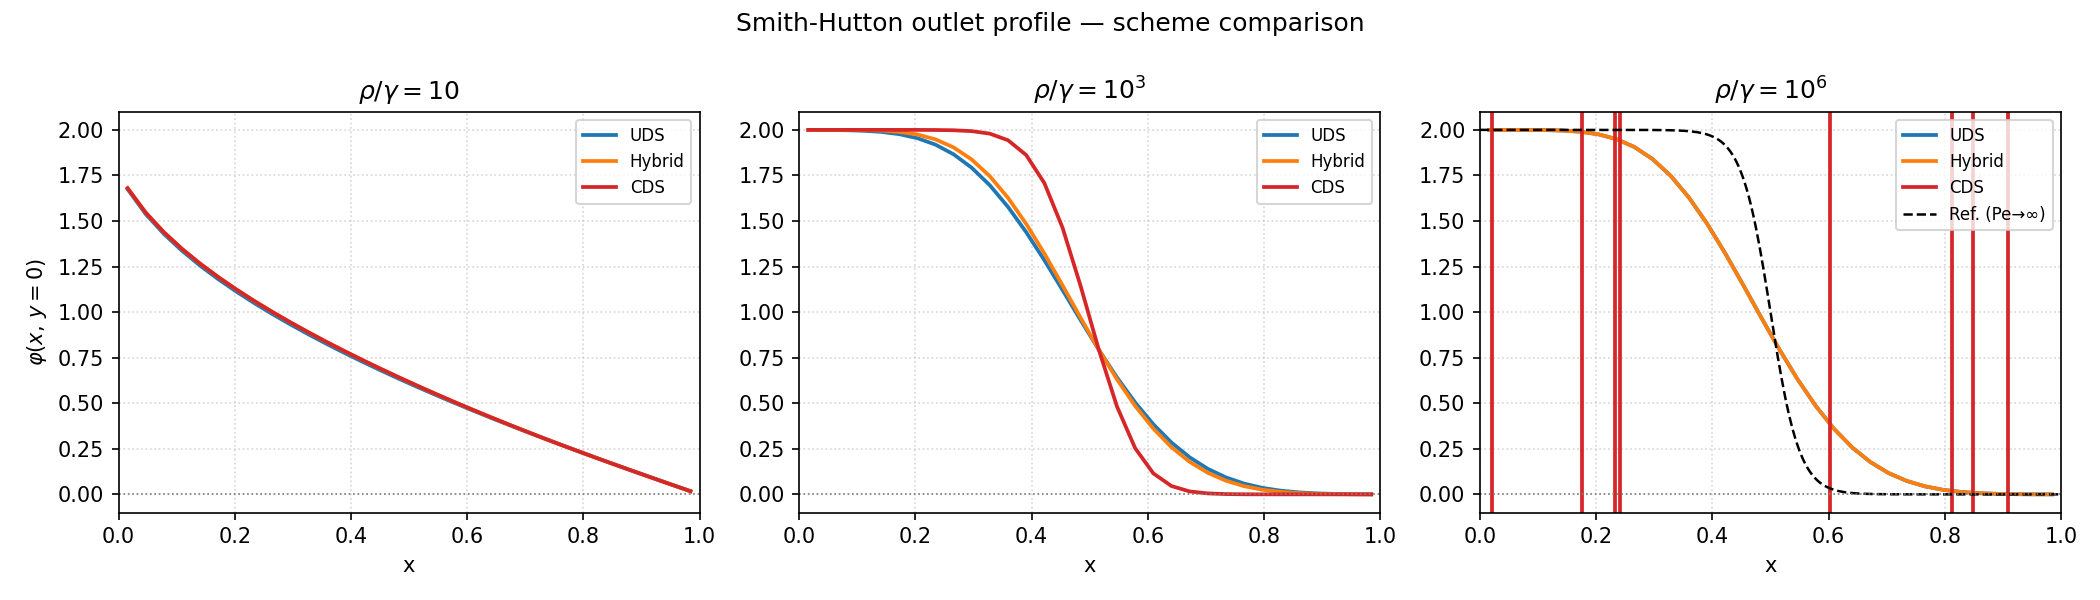
\includegraphics[width=\linewidth]{Chapter2/Media/SHSchemeComparison.png}
    \caption{Exit profile $\phi(x, 0)$ for CDS, UDS, and Hybrid compared against the reference of Smith and Hutton~\cite{SmithHutton1982} at each $\rho/\Gamma$ case. For $\rho/\Gamma = 10^6$ the reference corresponds to the $Pe \to \infty$ limit.}
    \label{figConvSH}
\end{figure}

\begin{figure}[ht]
    \centering
    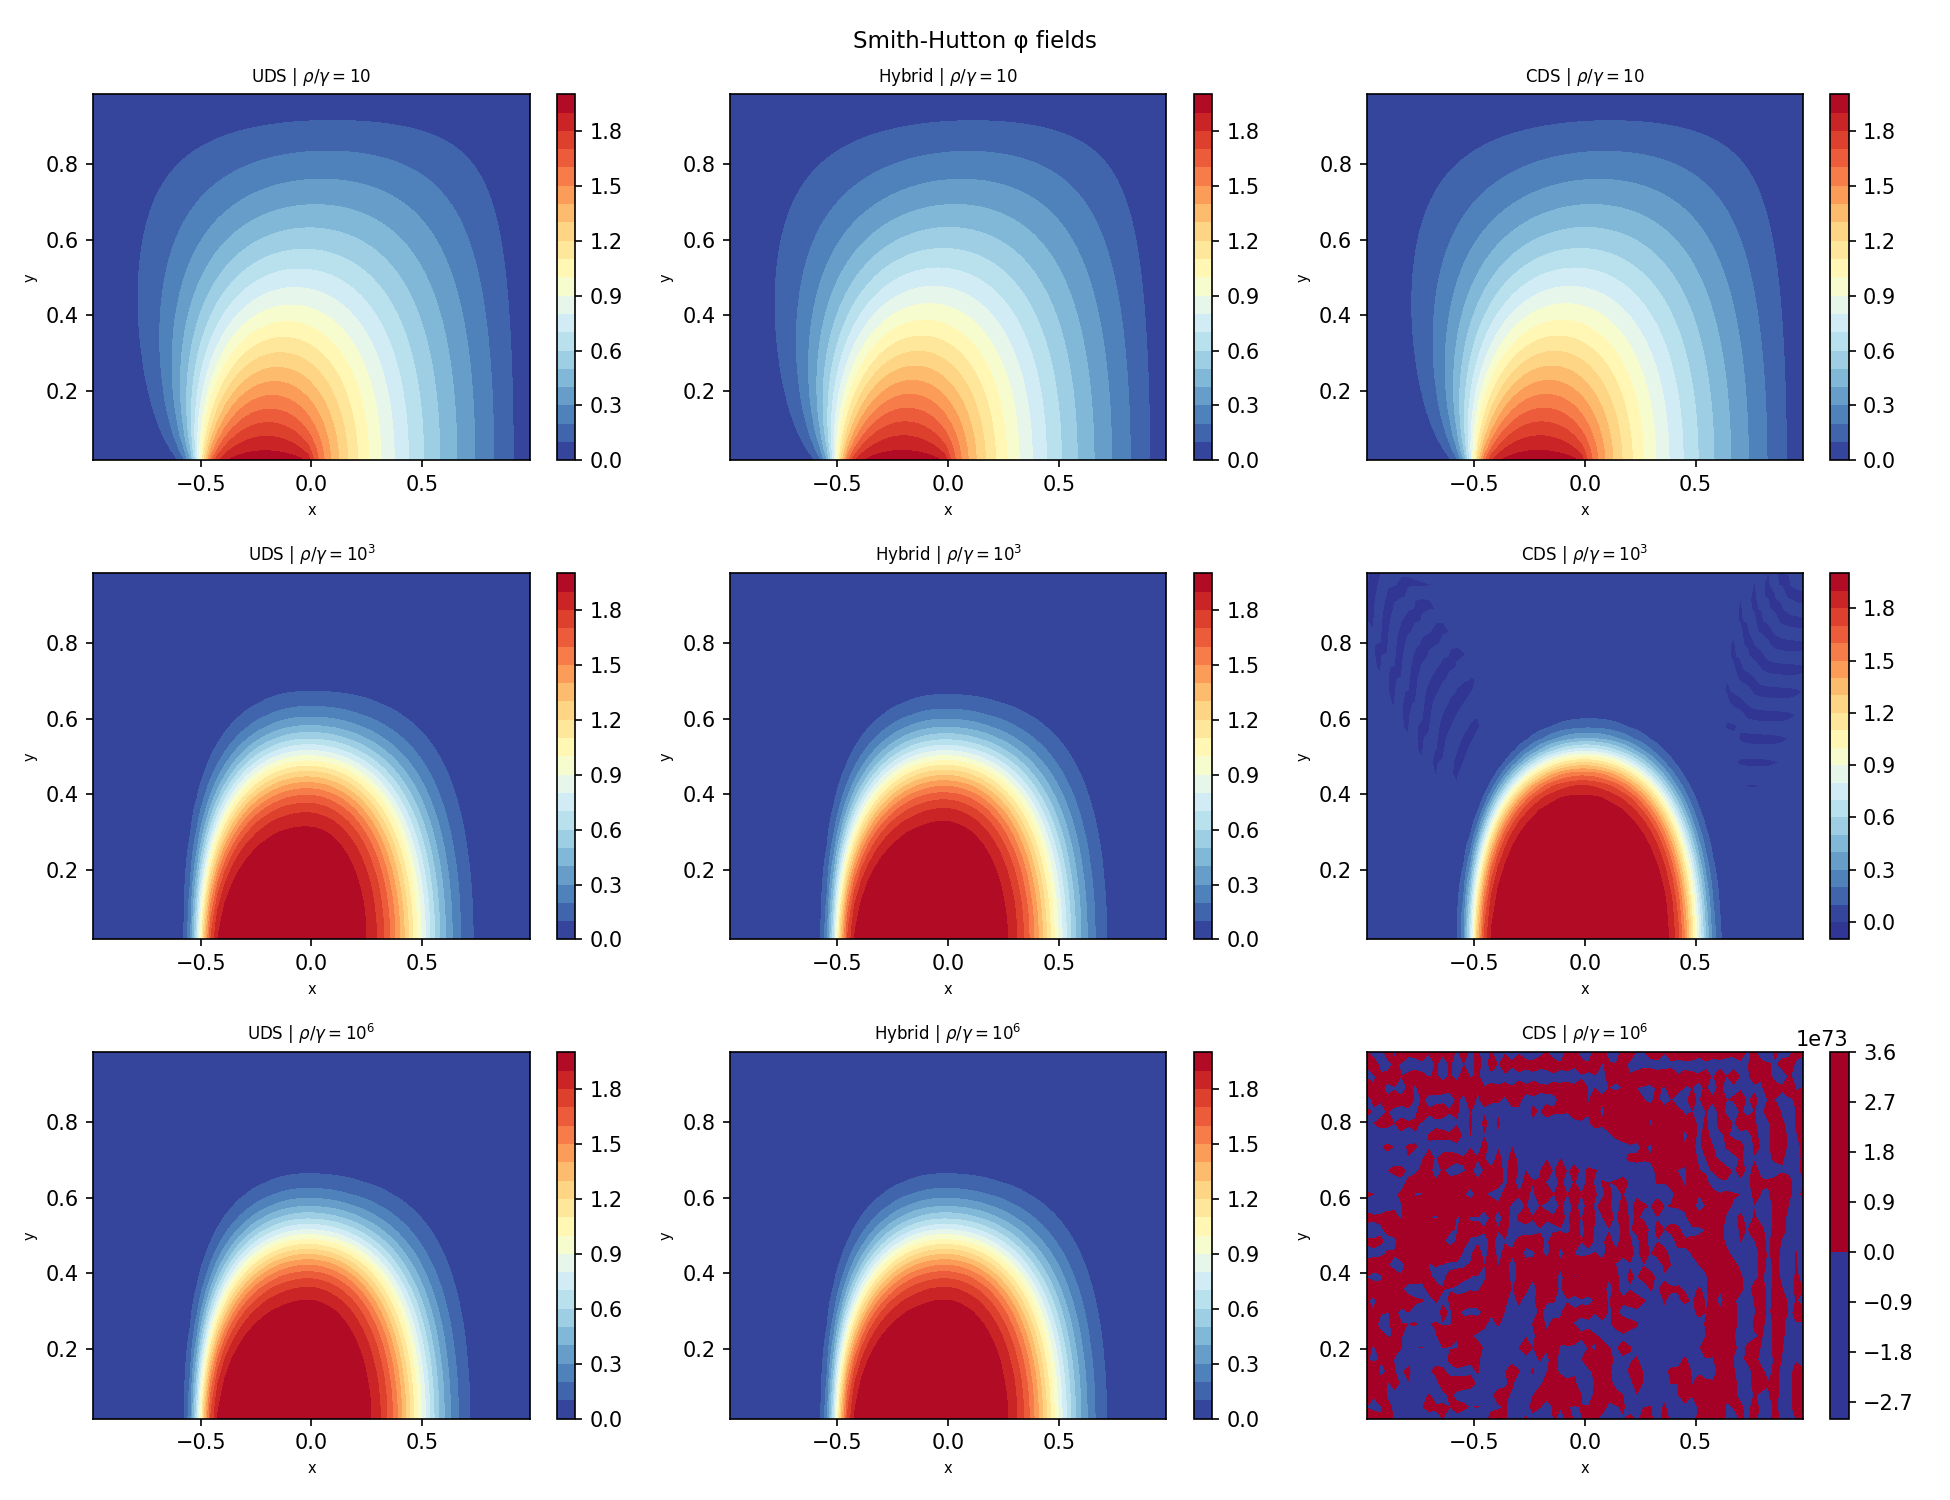
\includegraphics[width=\linewidth]{Chapter2/Media/SHSchemeFields.png}
    \caption{Steady-state $\phi$ field for UDS (left column), Hybrid (centre column), and CDS (right column) across all three $\rho/\Gamma$ cases (rows). At $\rho/\Gamma = 10^6$ the CDS solution has diverged and is shown at the scale of the numerical overflow.}
    \label{figConvUDS}
\end{figure}
